\documentclass[11pt]{beamer}
\usetheme{Warsaw}
\usepackage[utf8]{inputenc}
\usepackage[spanish]{babel}
\usepackage{amsmath}
\usepackage{amsfonts}
\usepackage{amssymb}
\usepackage{graphicx}
\author{N.Pérez-Medina}
\title{Capítulo 6 - Autosimilitud: dimensiones}
\setbeamercovered{transparent} 
\setbeamertemplate{navigation symbols}{} 
\logo{
\includegraphics[scale=0.04]{logo_fing_uach_bn.png} } 
\institute{\textbf{FING - UACH}
	\\
	\begin{small}
	\textit{Resumen del libro 'Análisis de series de tiempo no lineales' de Kantz y Schreiber}\\
	\end{small}
	
	\bigskip
	
	\begin{small}
	\textbf{Catedrático:} Dr. José Luis Herrera Aguilar
	\end{small}		
	} 
\date{\today} 
\subject{Series de tiempo} 


% Para tener un morado coqueto
\definecolor{lightPurple}{RGB}{186, 146, 209} % Morado claro
\definecolor{darkPurple}{RGB}{98, 54, 150}    % Morado oscuro
\setbeamercolor{structure}{fg=darkPurple} % Color principal para estructuras
\setbeamercolor{frametitle}{bg=darkPurple, fg=white} % Título del marco
\setbeamercolor{block title}{bg=darkPurple, fg=white} % Título de bloques
\setbeamercolor{block body}{bg=lightPurple!30, fg=black} % Cuerpo de bloques

\begin{document}

\begin{frame}
\maketitle
\end{frame}

\begin{frame}
\tableofcontents
\end{frame}

\section{Geometría del atractor y fractales}
\begin{frame} 
\tableofcontents[currentsection] % Solo muestra la sección actual
\end{frame}

\begin{frame}{Sobre el \textbf{\textit{Atractor}}}

\begin{block}{\textbf{\textit{Atractor}}}
	Conjunto en el \textit{espacio de fases} formado por las trayectorias no transitorias del sistema.
\end{block}

\begin{block}{Razón de su importancia}
	La \textit{sensibilidad a las condiciones iniciales} tiene su manifestación equivalente en la \textit{geometría} del \textbf{\textit{Atractor}}
\end{block}
\begin{block}{\textit{Extraños}}
Los \textbf{\textit{atractores}} de sistemas caóticos disipativos generalmente tienen una geometría muy complicada, lo que llevó a llamarlos \emph{extraños}.
\end{block}
\end{frame}

\begin{frame}{Sobre los \textit{Extraños}}
\begin{block}{Más adelante veremos}
	\begin{itemize}
		\item Los atractores \textit{extraños} con \textbf{\textit{dimenciones fraccionarias}} son típicos de los sistemas caóticos.
		\item Se asignan \textbf{\textit{dimenciones fraccionarias}} a objetos geométricos que exhiben una especie de \textbf{\textit{autosimilitud}}
	\end{itemize}
\end{block}

\end{frame}

\begin{frame}{Sobre la \textbf{\textit{autosimilitud}}(1/2)}
\centering
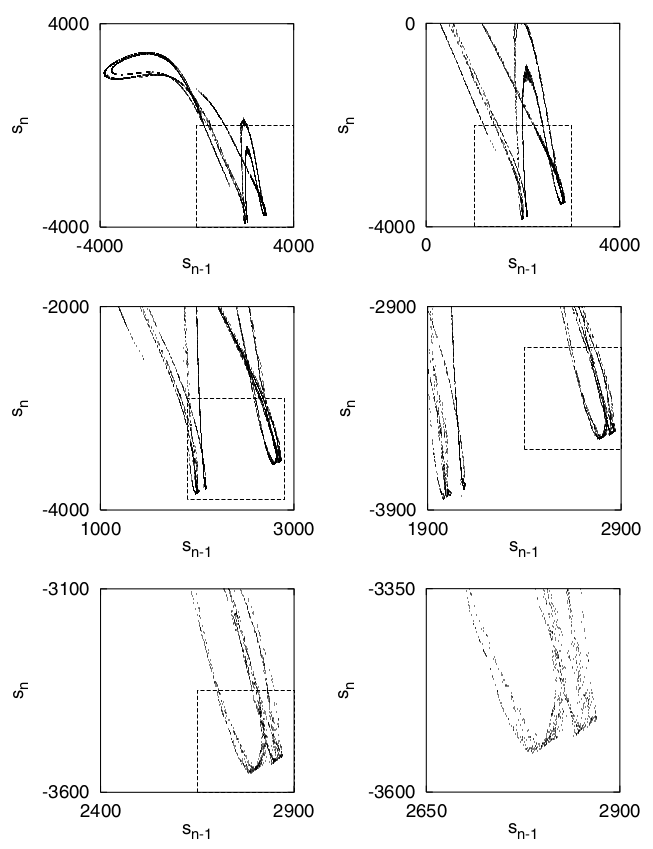
\includegraphics[scale=0.4]{autosimi.png} 
\end{frame}

\begin{frame}{Sobre la \textbf{\textit{autosimilitud}}2/2}
\centering
\medskip
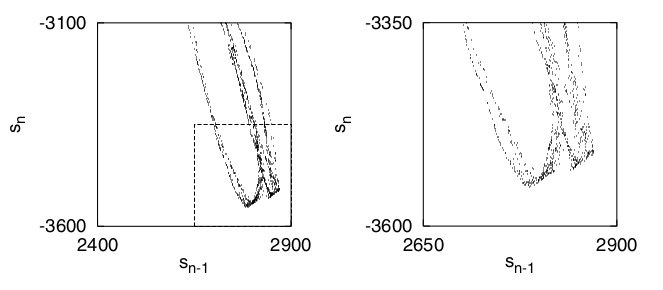
\includegraphics[scale=0.5]{autosimi2.png} 
\end{frame}

\section{Dimensión de correlación}
\begin{frame} 
\tableofcontents[currentsection] % Solo muestra la sección actual
\end{frame}

\begin{frame}{En general}
\begin{block}{Dimención de correlación}
	Es una definición de particular interés en aplicaciones prácticas donde el objeto geométrico debe ser reconstruido a partir de una muestra finita de datos\footnote{que probablemente contenga algunos errores también.}. Fue introducida por \textit{Grassberger} y \textit{Procaccia} (1983) y (1983a).
\end{block}
\end{frame}

\begin{frame}{Primero que nada}
\begin{block}{\textbf{\textit{Suma de correlación}} para una colección de puntos $\mathbf{x}_i$}
Es la fracción de todos los pares posibles de puntos que están más cerca de una distancia dada \(\epsilon\) en una norma particular.
\begin{equation}
C(\epsilon) = \frac{2}{N(N-1)} \sum_{i=1}^N \sum_{j=i+1}^N \Theta(\epsilon - || \mathbf{x}_i - \mathbf{x}_j ||),
\end{equation}
donde \(\Theta\) es la función escalón de Heaviside, \(\Theta(x) = 0 \ \text{si} \ x \leq 0\) y \(\Theta(x) = 1 \ \text{para} \ x > 0\).
\end{block}
\end{frame}

\begin{frame}{Ahora sí}
\begin{block}{\textit{\textbf{Dimención de correlación}}}
En el límite de una cantidad infinita de datos (\(N \rightarrow \infty\)) y para valores pequeños de \(\epsilon\), esperamos que \(C\) escale como una ley de potencia, \(C(\epsilon) \sim \epsilon^D\), y podemos definir la \textbf{\textit{dimensión de correlación}} \(D\) por:

\begin{equation}
d(N, \epsilon) = \frac{\partial \ln C(\epsilon, N)}{\partial \ln \epsilon}, 
\end{equation}

\begin{equation}
D = \lim_{\epsilon \to 0} \lim_{N \to \infty} d(N, \epsilon).
\end{equation}
\end{block}

\end{frame}

\begin{frame}{Consideraciones}
\begin{block}{Siempre que tengamos una \textit{muestra finita}}
\begin{itemize}
	\item \(N\) está limitado por el tamaño de la muestra
	\item El rango de elecciones significativas de \(\epsilon\) está limitado por la precisión de los datos
\end{itemize}
\end{block}
\begin{block}{Requisitos prácticos para la estimación de la dimensión}
\begin{itemize}
\item Aunque la \textbf{\textit{dimensión de correlación}} es \textit{invariante}, la \textbf{\textit{suma de correlación}} en una escala dada \(\epsilon_0\) no lo es.
\item La \textit{\textbf{dimensión de correlación}} es una herramienta para cuantificar la auto-similitud\textbf{ cuando se sabe que está presente.}
\end{itemize}
\end{block}
\end{frame}

\section{Suma de correlación a partir de una serie temporal}
\begin{frame} 
\tableofcontents[currentsection] % Solo muestra la sección actual
\end{frame}

\begin{frame}{Sobre la \textbf{\textit{Suma de correlación}}}
\begin{block}{En general}
\begin{itemize}
\item Un valor para el tiempo de retardo que produzca un retrato de fase \textit{convincente} debería servir también para la \textbf{\textit{suma de correlación}}.
\item Los resultados son invariantes bajo cambios \textit{razonables} en el procedimiento de \textit{incrustación}.
\end{itemize}
\end{block}
\end{frame}

\begin{frame}{\textbf{\textit{Algoritmo de correlación}}}
\begin{block}{Descripción general}
\begin{enumerate}
\item Determinar la suma de correlación $C(m, \epsilon)$, para el rango de $\epsilon$ disponible y para varias dimensiones de incrustación $m$.
\item Inspeccionar $C(m, \epsilon)$ en busca de signos de \textbf{\textit{autosimilaridad}}.
\item Si estas señales son lo suficientemente convincentes, podemos calcular un valor para la \textbf{\textit{dimensión de correlación}}.
\end{enumerate}
Los pasos requieren cierto cuidado con el fin de evitar resultados erróneos o engañosos. 
\end{block}
\end{frame}

\begin{frame}{Sobre las \textbf{\textit{correlaciones temporales}}}
\begin{block}{\textbf{\textit{Correlaciones temporales}}}
Los vectores de incrustación en tiempos sucesivos suelen estar también cercanos en el espacio de fases debido a la evolución continua del tiempo. A este tipo de correlaciones las llamamos \textbf{\textit{correlaciones temporales}}.
\end{block}
\begin{block}{Relevancia}
\begin{itemize}
\item Muchos métodos cuantitativos de análisis de series temporales pueden verse sesgados por \textbf{\textit{correlaciones temporales.}} 
\item En el caso de la \textbf{\textit{dimensión de correlación}}, esto conduce a una subestimación seria\footnote{a menos que se tenga el cuidado necesario.} 
\end{itemize}
\end{block}
\end{frame}

\begin{frame}{Solución simple}
\small
\begin{block}{Idea central}
\textit{Excluir} aquellos pares de puntos que están cercanos, \textbf{no} por la geometría del atractor, sino porque están correlacionados.
\end{block}
\begin{block}{Entonces}
La segunda suma comienza solo después de que haya transcurrido un intervalo de tiempo típico $t_{\min} = n_{\min} \Delta t$:

\begin{equation}
C(m, \epsilon) = \frac{2}{(N - n_{\min})(N - n_{\min} - 1)} \sum_{i=1}^{N} \sum_{j=1, j \neq i + t_{\min}}^{N} \Theta(\epsilon - \| \mathbf{s}_i - \mathbf{s}_j \|) \,.
\end{equation}

La función escalón $\Theta$ cuenta 1 si los puntos están a menos de $\epsilon$ pero sólo se consideran pares con separación temporal mayor o igual a $t_{\min}$.
\end{block}
\end{frame}

\section{Interpretación y dificultades}
\begin{frame} 
\tableofcontents[currentsection] % Solo muestra la sección actual
\end{frame}

\begin{frame}{Consideraciones necesarias}
\small
\begin{block}{En general}
\begin{itemize}
\item La cantidad que puede calcularse con un procedimiento más o menos automatizado es la \textbf{\textit{suma de correlación}} $C(m, \epsilon)$
\item Una \textit{\textbf{dimensión de correlación}} solo puede asignarse como resultado de una cuidadosa \textit{interpretación} de estas curvas.
\item Una estimación de una \textbf{\textit{dimensión de correlación}} implica una extrapolación no trivial desde un conjunto de datos finito hacia un atractor que \textit{supuestamente} existe.
\item Existen características que podemos esperar encontrar en una \textbf{\textit{suma de correlación}} típica para una muestra tomada de un \textit{atractor extraño.}
\end{itemize}
\end{block}
\end{frame}


\begin{frame}{Pendientes locales $D(m,\epsilon)$}
\centering
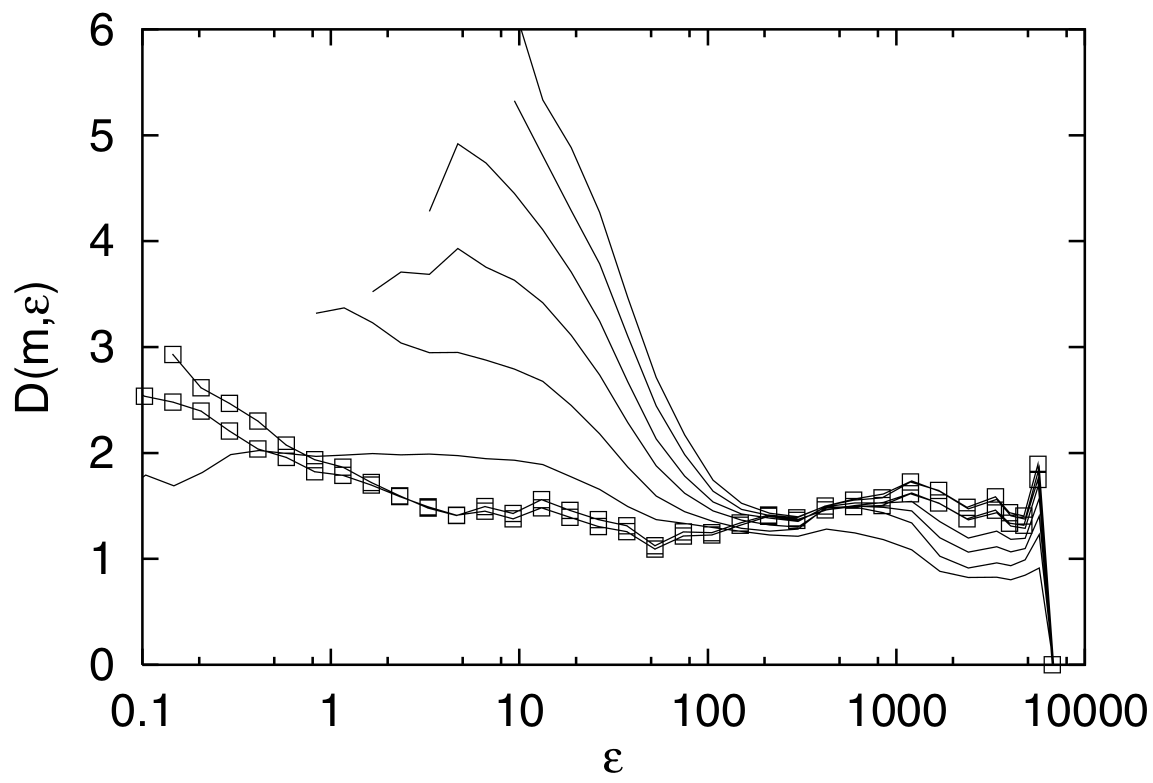
\includegraphics[scale=0.25]{dme.png} 
\end{frame}


\begin{frame}{Sobre la \textit{region de escalamiento}}
\begin{block}{En general}
\begin{itemize}
\item Una señal determinista de baja dimensión, medida con un error relativo mayor a aproximadamente 2--3\%, \textbf{no} mostrará una \textit{región de escalamiento} significativa de $C(m, \epsilon)$ (ni una meseta de $D(m, \epsilon)$)
\item Incluso datos deterministas de muy buena calidad pueden carecer de una \textit{región de escalamiento}
\item Una \textit{región de escalamiento} siempre debe establecerse por \textbf{inspección}. 
\end{itemize}
\end{block}
\end{frame}

\begin{frame}{Hasta ahora}
\begin{block}{La esperanza es:}
Encontrar \textit{firmas} que reconozcamos como \textbf{típicas} de sistemas deterministas y así justificar el enfoque \textit{a posteriori}, un concepto \textbf{\textit{peligroso}.}
\end{block}

\end{frame}

\section{Señales multi-escala o auto-similares}
\begin{frame} 
\tableofcontents[currentsection] % Solo muestra la sección actual
\end{frame}
\subsection{Leyes de escalamiento}

\begin{frame}{Idea gráfica}
\centering
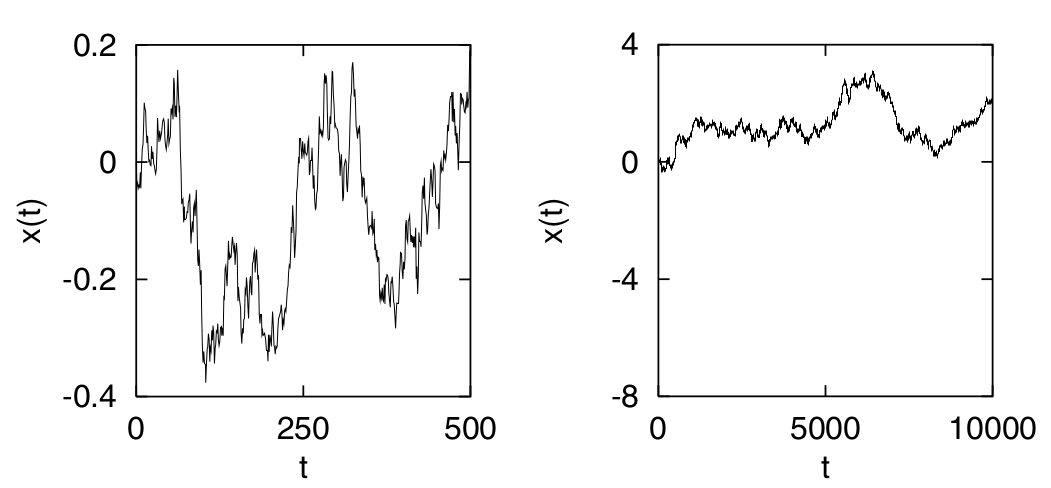
\includegraphics[scale=0.3]{compara-escalas.png} 
\end{frame}

\begin{frame}{Más términos}
\begin{block}{Autosimilitud}
Una señal o figura es \textit{autosimilar} si luce igual bajo una transformación de escala \textbf{igual} en todos los ejes.
\end{block}

\begin{block}{Autoafinidad}
Una señal es \textit{autoafín} si luce igual bajo una transformación \textbf{desigual} de escala en cada eje. La forma se conserva estadísticamente si se escala de la forma:

\begin{equation}
\langle \Delta x^2 \rangle \propto \Delta t^{2H},
\end{equation}

donde al exponente $H$ le llamamos \textbf{\textit{exponente de Hurst.}}
\end{block}

\end{frame}

\begin{frame}{Exponente de Hurst}
\begin{block}{En general}
\begin{itemize}
	\item Es un número entre 0 y 1 que caracteriza el grado de dependencia temporal 
	\item Nos dice qué tan correlacionados están los cambios a través del tiempo
	\item Indica cómo crece la varianza de los incrementos $(x(t+\Delta t)-x(t))^2$ al aumentar $\Delta t$.
	
\end{itemize}
\medskip
$$
\langle \Delta x^2 \rangle \propto \Delta t^{2H}
$$
\end{block}
\end{frame}

\begin{frame}{Sobre sus valores y la \textit{memoria}}
\begin{block}{En resumen}
\begin{center}
\small
\begin{tabular}{|c|p{6cm}|}
\hline
\textbf{Valor de \( H \)} & \textbf{Interpretación} \\
\hline
\( H = 0.5 \) & Los incrementos son \textbf{no correlacionados}, es decir, no hay \textit{memoria} en la serie.\\
\hline
\( H > 0.5 \) & \textbf{Persistencia}: si la serie sube, tiende a seguir subiendo; si baja, tiende a seguir bajando. Hay \textbf{memoria positiva} y correlación a largo plazo.\\
\hline
\( H < 0.5 \) & \textbf{Antipersistencia}: si la serie sube, tiende a revertirse y bajar. Hay \textbf{memoria negativa} o tendencia a alternar los cambios.\\
\hline
\end{tabular}
\end{center}
\end{block}

\end{frame}

\subsection{Análisis de fluctuación sin tendencia}

\begin{frame}{Planteando un nuevo problema}
\small
\begin{block}{Contextualización}
En teoría, la relación:
$$
\langle \Delta x^2 \rangle \propto \Delta t^{2H}
$$

sirve para estimar el \textbf{\textit{exponente de Hurst}}, pero en la práctica los datos reales tienen problemas:
\begin{itemize}
	\item Tendencias (por ejemplo, crecimiento lento en media).
	\item Ruido.
	\item Cambios de régimen (no estacionariedad).
	\item Saturación por límites de resolución (como en mediciones físicas).
\end{itemize}

Por eso \textbf{no se puede simplemente calcular varianzas sobre incrementos y esperar obtener un Hurst confiable.}
\end{block}
\end{frame}

\begin{frame}{Alternativa para solucionarlo}
\begin{block}{Analísis de fluctuación sin tendencia (DFA)}
 En general, el DFA elimina el efecto de tendencias lentas para enfocarse en las fluctuaciones de la señal
\end{block}
\end{frame}

\begin{frame}{\textbf{DFA} Paso a paso (1/3)}
\begin{block}{\textbf{Paso 1} Construir la señal integrada}
Primero se transforma la señal original $x(t)$ en una \textit{señal acumulativa} o 'camino integrado'
\begin{equation}
y(t) = \int_{0}^{t} (x(t') - \bar{x}) dt',
\end{equation}
\end{block}
\end{frame}

\begin{frame}{\textbf{DFA} Paso a paso (2/3)}
\begin{block}{\textbf{Paso 2} Dividir en ventanas y eliminar la tendencia local}
Se divide la señal integrada $y(t)$ en ventanas de longitud $\tau$ y en cada ventana se ajusta un polinomio de grado $k$ que representa la \textit{tendencia local} $g^{(k)}(t)$

Esa tendencia se resta para obtener las fluctuaciones sin tendencia
\begin{equation}
v^{(k)}(\tau)=\text{RMS}[y(t)-g^{(k)}(t)]
\end{equation}

Donde \textit{RMS} es la raíz cuadrada del promedio cuadrático de los residuos.
\end{block}

\end{frame}


\begin{frame}{\textbf{DFA} Paso a paso (3/3)}
\begin{block}{\textbf{Paso 3} Escalamiento de la fluctuación}
Después se calcula cómo crece esa fluctuación $v^{(k)}(\tau)$ con el tamaño de ventana $\tau$
\begin{equation}
\langle v^{(k)}(\tau) \rangle \propto \tau^{2+2H}
\end{equation}
Este crecimiento es el que da el \textbf{\textit{exponente de Hurst}}
\end{block}
\end{frame}


\section*{Gracias}
\begin{frame} 
\tableofcontents[currentsection] % Solo muestra la sección actual
\end{frame}

\begin{frame}{Por su atención}
\centering
\begin{Huge}
Gracias y arriba los pumas
\end{Huge}

\includegraphics[scale=0.3]{goyo.jpeg} 
\end{frame}
\end{document}
